% Vayu Console — technical document for judges.
%
% Build:  pdflatex -interaction=nonstopmode technical-document.tex   (run twice)
%
% Deliberately light-background rather than matching the product's black theme.
% This is fifteen pages of dense prose meant to be read and printed; a black page
% is hostile to both. The palette appears in the title page and the accents.
\documentclass[11pt,a4paper]{article}

\usepackage[T1]{fontenc}
\usepackage[utf8]{inputenc}
\usepackage{textcomp}
% Latin Modern. Charter and the newtx/mathdesign families declare .sty files in
% this TeX install but ship no font metrics, so they fail at load time rather
% than at package time. lmodern is present in full and renders cleanly at 11pt.
\usepackage{lmodern}
\usepackage{microtype}
\usepackage[margin=2.2cm,top=2.0cm,bottom=2.2cm]{geometry}
\usepackage{graphicx}
\usepackage{xcolor}
\usepackage{booktabs}
\usepackage{tabularx}
\usepackage{longtable}
\usepackage{enumitem}
\usepackage{titlesec}
\usepackage{fancyhdr}
\usepackage{amsmath}
\usepackage{tikz}
\usepackage{caption}
\usepackage[hidelinks]{hyperref}
\usetikzlibrary{arrows.meta,positioning,fit,backgrounds,calc}

% --- Palette, from the product's globals.css --------------------------------
\definecolor{vblack}{HTML}{0A0A0A}
\definecolor{vamber}{HTML}{B45309}   % darkened for contrast on white
\definecolor{vgreen}{HTML}{15803D}
\definecolor{vred}{HTML}{B91C1C}
\definecolor{vgrey}{HTML}{52525B}
\definecolor{vline}{HTML}{D4D4D8}
\definecolor{vwash}{HTML}{F4F4F5}

\hypersetup{colorlinks=true,linkcolor=vamber,urlcolor=vamber,
  pdftitle={Vayu Console — Technical Document},
  pdfauthor={singhpranav431}}

% --- Structure --------------------------------------------------------------
\titleformat{\section}{\normalfont\Large\bfseries\color{vblack}}{\thesection}{0.7em}{}
\titleformat{\subsection}{\normalfont\large\bfseries\color{vblack}}{\thesubsection}{0.6em}{}
\titlespacing*{\section}{0pt}{1.3ex plus .5ex}{0.6ex}
\titlespacing*{\subsection}{0pt}{1.0ex plus .3ex}{0.4ex}

\pagestyle{fancy}\fancyhf{}
\renewcommand{\headrulewidth}{0.4pt}
\fancyhead[L]{\footnotesize\color{vgrey}Vayu Console \textemdash{} Technical Document}
\fancyhead[R]{\footnotesize\color{vgrey}\thepage}

\setlist[itemize]{leftmargin=1.2em,itemsep=0.25ex,topsep=0.5ex}
\setlist[enumerate]{leftmargin=1.5em,itemsep=0.25ex,topsep=0.5ex}
\captionsetup{font=small,labelfont=bf,labelsep=period}
\renewcommand{\arraystretch}{1.12}

% A pulled-out statement. Used sparingly, for claims the whole document rests on.
\newcommand{\keyclaim}[1]{%
  \par\vspace{0.7ex}\noindent
  \colorbox{vwash}{\parbox{\dimexpr\linewidth-2\fboxsep}{%
    \color{vblack}\textbf{#1}}}%
  \par\vspace{0.9ex}}

\newcommand{\code}[1]{\texttt{\small #1}}
\newcommand{\NOx}{NO\textsubscript{2}}
\newcommand{\SOx}{SO\textsubscript{2}}
\newcommand{\PM}{PM\textsubscript{2.5}}
\newcommand{\ugm}{\textmu g/m\textsuperscript{3}}

\begin{document}

% ===========================================================================
% Title page
% ===========================================================================
\begin{titlepage}
\pagecolor{vblack}\color{white}
\thispagestyle{empty}
\vspace*{3.2cm}

{\footnotesize\bfseries\color{vamber!85!white}\hspace{1pt} ET AI HACKATHON 2.0\par}
\vspace{0.9cm}
{\fontsize{46}{50}\selectfont\bfseries Vayu Console\par}
\vspace{0.5cm}
{\LARGE\color{vline} From pollution signals to defensible action\par}
\vspace{0.4cm}
{\large\color{vgrey!60!white} Urban Air Quality Decision Intelligence\par}

\vspace{1.4cm}
{\color{vamber!85!white}\rule{5cm}{1.2pt}}
\vspace{1.2cm}

{\Large\bfseries Technical Document\par}
\vspace{0.35cm}
{\normalsize\color{vline} A detailed account of the system, its evidence,\\
and the claims it deliberately refuses to make.\par}

\vfill
{\footnotesize\color{vgrey!70!white}
Team \textbf{\color{white}singhpranav431}\\[0.3em]
Category: Urban Air Quality Decision Intelligence / Environmental Decision Support\\[0.3em]
\href{https://vayu-console-web.vercel.app/console}{\color{vamber!85!white}vayu-console-web.vercel.app/console}
\quad\textbullet\quad
\href{https://github.com/Pranavsingh431/vayu_console}{\color{vamber!85!white}github.com/Pranavsingh431/vayu\_console}
\par}
\end{titlepage}
\nopagecolor\color{black}

\tableofcontents
\thispagestyle{fancy}
\vspace{1em}

\noindent\small\color{vgrey}
Every quantitative claim in this document is traceable to the repository or to the
live API. Where a result has not been measured, it says so. Section~\ref{sec:limits}
is the honest list of what the system cannot do, and it is not short.
\color{black}\normalsize

\newpage

% ===========================================================================
\section{Executive Summary}

Delhi has no shortage of air quality dashboards. Every one of them answers the same
question: how bad is the air right now. That is not the question a municipal officer
has to answer at 2\,a.m. during a severe episode. Their question is what to
\emph{do}, and how to defend that decision in a review meeting the following
morning.

Vayu Console is a decision support system for that gap. It takes an observed
pollution episode at a monitoring station and runs it through four stages:
\textbf{situation}, \textbf{evidence}, \textbf{decision}, \textbf{explanation}. It
evaluates three independent hypotheses for what may be contributing, rates the
evidence for each one against observations that are, where possible, collected
independently of the monitor being explained, applies deterministic policy rules to
that evidence, and exposes the complete audit trace behind every recommendation it
produces.

\keyclaim{The defining design decision is that the system is allowed to return
``insufficient evidence'' and recommend nothing at all.}

That is not an error path or an unhandled case. It is a first-class output with its
own visual treatment and its own copy, because the alternative is worse: a system
that always answers will, on the many station-hours where the required observations
are missing, produce an answer indistinguishable from one that is grounded. An
officer cannot tell the two apart. That is not a gap in a user interface, it is a
system that lies at a known rate.

Three things are worth a technical reader's attention before the detail.

\begin{enumerate}
  \item \textbf{This is source-contribution screening, not source apportionment.}
  Delhi's regulatory network measures mass concentration, not chemical composition.
  Without speciation there is no ground truth for attribution, so any percentage
  this system emitted would be invented. It emits none. There is no pie chart, no
  stacked bar, and no \ugm{} figure attributed to any source anywhere in the
  product.

  \item \textbf{A supervised source classifier was built, scored 98.6\% accuracy,
  and was deleted.} Its labels were generated by a rule over its own input
  features, so it had learned the rule rather than the atmosphere. The instructive
  part is that every instrument we could have pointed at it for honesty --- SHAP,
  conformal prediction, calibration curves --- would have corroborated the
  fabrication rather than exposed it. Section~\ref{sec:classifier} sets out the
  measurement and the argument.

  \item \textbf{One validation has been run to completion.} The COVID-19 lockdown
  calibrated and accepted the traffic module at a likelihood ratio of 2.11, which
  is ``weak'' on the Kass \& Raftery scale, and the module is capped in code
  because of it. The other declared tests are pending, the engine reports them as
  pending at \code{/evidence/history}, and the console shows them as pending.
  Section~\ref{sec:validation} does not round any of them up.
\end{enumerate}

% ===========================================================================
\section{Problem Statement}

A municipal air quality officer in Delhi during a severe episode has access to a
real-time \PM{} reading from a network of monitoring stations, and to public AQI
dashboards that render that reading with a colour and a category label. What they
do not have is any structured answer to the questions that actually determine their
next action:

\begin{itemize}
  \item Why is this happening, and what evidence supports each candidate
  explanation?
  \item Which of the available interventions is proportionate to that evidence?
  \item How confident should anyone be in that judgement?
  \item If challenged tomorrow, what exactly is the reasoning, and where are its
  weaknesses?
\end{itemize}

None of these are measurement problems. The measurement exists. They are reasoning
problems, and at present they are solved by an officer manually correlating
fragmented signals --- a station reading here, a news report of stubble burning
there, a sense of the wind --- under time pressure, with no record of how the
conclusion was reached.

\keyclaim{The gap is not between data and dashboards. It is between a reading and a
decision an officer can defend.}

% ===========================================================================
\section{Problem Analysis and Motivation}

The obvious response to this gap is to build a model that predicts the pollution
source, attach a confidence score, and present the result. That approach fails for
a reason specific to the data, and understanding the reason shaped the entire
system.

\subsection{There is no ground truth for attribution}

Identifying which source produced a given mass of \PM{} is called \emph{source
apportionment}. It is a mature field, and it works by chemical speciation:
collecting filter samples, measuring the elemental and organic composition, and
solving a receptor model such as Chemical Mass Balance or Positive Matrix
Factorisation against known source profiles.

Delhi's regulatory network does not do this. It measures mass concentration
(\PM{}, PM\textsubscript{10}) and a handful of gaseous species (\NOx{}, \SOx{},
CO, O\textsubscript{3}). There is no composition data, and therefore no labelled
dataset of ``this station-hour was caused by vehicles'' anywhere in the archive ---
because producing one would itself require the apportionment we are trying to
perform.

This has a hard consequence. A supervised model needs a target. If no target
exists, one must be invented, and any invented target is a function of the same
features the model will be given. Section~\ref{sec:classifier} shows what happens
when you do that anyway.

\subsection{What is available instead}

The asymmetry that makes the system possible is that \emph{some} hypotheses have
evidence that exists outside the measurement being explained, and some do not.

Satellites observe agricultural fires in Punjab and Haryana independently of any
Delhi air quality monitor. That observation is exogenous: it cannot be a
restatement of the thing it is being used to explain. Traffic has no such signal
--- there is no satellite watching Delhi's cars --- so its only signature lies in
the same chemistry we would be reasoning from. Industry has neither an exogenous
signal nor a natural experiment that isolates it.

This asymmetry is not a nuisance to be smoothed over. It is reported as a
first-class property called \emph{identification}, separately from evidence
strength, because it does not vary hour to hour. It is a statement about what can
be known at all.

\subsection{Why historical events rather than live data}

Live data cannot validate a reasoning system. You produce a recommendation and
never find out whether it was right, because the counterfactual is unobservable.

Historical episodes in which a known external intervention changed one input while
leaving others in place are the only setting where the logic can be tested. The
COVID-19 lockdown drove traffic to approximately zero by government order, which
makes $P(\NOx \mid \text{vehicles} \approx 0)$ directly observable rather than
assumed. No researcher could run that experiment deliberately.

The console therefore replays reconstructed historical incidents, and says so on
every screen.

% ===========================================================================
\section{Proposed Solution: Vayu Console}

Vayu Console implements a four-stage pipeline, and its interface is laid out in
that order because the layout \emph{is} the workflow.

\begin{center}
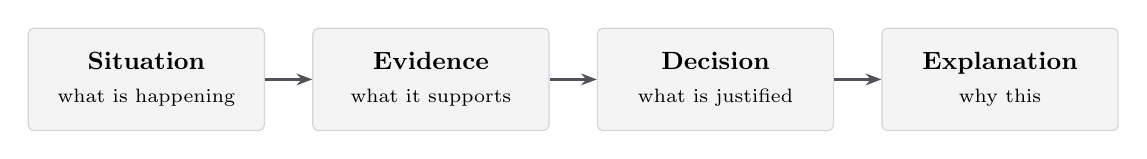
\begin{tikzpicture}[
  node distance=6mm,
  stage/.style={draw=vline,fill=vwash,rounded corners=2pt,minimum height=13mm,
                minimum width=30mm,align=center,font=\small},
  arr/.style={-{Stealth[length=2mm]},draw=vgrey,thick}]
  \node[stage] (a) {\textbf{Situation}\\[1pt]\scriptsize what is happening};
  \node[stage,right=of a] (b) {\textbf{Evidence}\\[1pt]\scriptsize what it supports};
  \node[stage,right=of b] (c) {\textbf{Decision}\\[1pt]\scriptsize what is justified};
  \node[stage,right=of c] (d) {\textbf{Explanation}\\[1pt]\scriptsize why this};
  \draw[arr] (a)--(b); \draw[arr] (b)--(c); \draw[arr] (c)--(d);
\end{tikzpicture}
\end{center}

\textbf{Situation} presents the measured concentration against the Central
Pollution Control Board's published \PM{} breakpoints. Severity is deliberately
\emph{not} derived from evidence strength: evidence says which explanation is
plausible, it says nothing about how bad the air is. An officer can cite a measured
number against a published threshold; they cannot cite a model output.

\textbf{Evidence} evaluates three hypotheses independently and reports, for each,
its strength, the quality of the data underneath it, its identification status, the
supporting and contradicting observations, the assumptions in play, and its
historical validation record.

\textbf{Decision} applies deterministic rules to the evidence report. The rule
engine may read nothing else. If a fact is not in the evidence report, no rule can
use it, which is what guarantees that every recommendation traces back to an
observation.

\textbf{Explanation} is the Challenge Recommendation interaction: one click on any
recommendation exposes the full trace from advice back to observation, including
the evidence that argues \emph{against} it.

\subsection{The architectural invariant}

\keyclaim{The Decision Engine consumes the Evidence Report and touches no raw data.}

This is enforced structurally rather than by convention. The decision layer's only
input type is \code{EvidenceReport}. It has no database session and no access to
station readings, satellite detections, or meteorology. The consequence is that no
rule can reach a recommendation that the evidence does not carry, and every
recommendation is reconstructible from a serialisable object.

% ===========================================================================
\section{System Architecture}

\begin{center}
\begin{tikzpicture}[
  font=\footnotesize,
  lay/.style={draw=vline,fill=white,rounded corners=2pt,minimum height=9mm,
              text width=105mm,align=center,inner sep=2mm},
  hot/.style={lay,draw=vamber,line width=0.8pt,fill=vamber!5},
  lbl/.style={font=\scriptsize\bfseries\color{vgrey},anchor=east},
  arr/.style={-{Stealth[length=2mm]},draw=vgrey}]

  \node[lay] (src) {OpenAQ S3 archive \textperiodcentered{} NASA FIRMS (VIIRS)
                    \textperiodcentered{} Open-Meteo};
  \node[lbl] at ($(src.west)+(-2mm,0)$) {SOURCES};

  \node[lay,below=5mm of src] (ing) {Ingestion \& validation: sentinel rejection,
        UTC normalisation, station deduplication};
  \node[lbl] at ($(ing.west)+(-2mm,0)$) {INGEST};

  \node[lay,below=5mm of ing] (db) {Supabase PostgreSQL + PostGIS};
  \node[lbl] at ($(db.west)+(-2mm,0)$) {STORE};

  \node[hot,below=5mm of db] (ev) {\textbf{Evidence Engine}\ \ \ biomass
        \textperiodcentered{} traffic \textperiodcentered{} industrial};
  \node[lbl] at ($(ev.west)+(-2mm,0)$) {EVIDENCE};

  \node[hot,below=5mm of ev] (de) {\textbf{Decision Engine}\ \ \ rules
        $\rightarrow$ policies $\rightarrow$ recommendations};
  \node[lbl] at ($(de.west)+(-2mm,0)$) {DECIDE};

  \node[lay,below=5mm of de] (api) {FastAPI (read-only JSON) $\rightarrow$
        Next.js Operations Console $\rightarrow$ Officer};
  \node[lbl] at ($(api.west)+(-2mm,0)$) {SERVE};

  \draw[arr] (src)--(ing); \draw[arr] (ing)--(db); \draw[arr] (db)--(ev);
  \draw[arr] (ev)--(de);  \draw[arr] (de)--(api);
\end{tikzpicture}
\captionof{figure}{System architecture. The two highlighted layers are where the
reasoning happens; everything above them is data handling and everything below is
delivery.}
\end{center}

The reasoning flow within those two layers, including the branch that produces no
recommendation at all:

\begin{center}
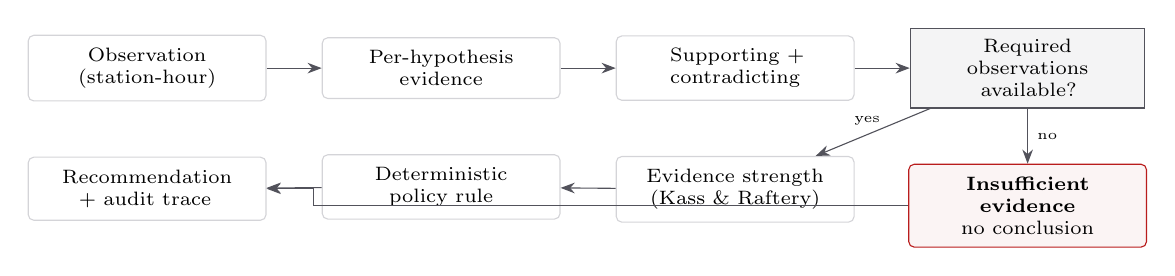
\begin{tikzpicture}[
  font=\scriptsize,
  n/.style={draw=vline,fill=white,rounded corners=2pt,align=center,inner sep=1.6mm,
            text width=27mm},
  d/.style={draw=vgrey,fill=vwash,align=center,inner sep=1.4mm,text width=27mm},
  stop/.style={n,draw=vred,fill=vred!5},
  arr/.style={-{Stealth[length=1.8mm]},draw=vgrey}]

  \node[n] (o) {Observation\\(station-hour)};
  \node[n,right=7mm of o] (h) {Per-hypothesis\\evidence};
  \node[n,right=7mm of h] (s) {Supporting +\\contradicting};
  \node[d,right=7mm of s] (q) {Required\\observations\\available?};

  \node[stop,below=7mm of q] (ins) {\textbf{Insufficient}\\\textbf{evidence}\\no conclusion};
  \node[n,below=7mm of s] (st) {Evidence strength\\(Kass \& Raftery)};
  \node[n,below=7mm of h] (r) {Deterministic\\policy rule};
  \node[n,below=7mm of o] (rec) {Recommendation\\+ audit trace};

  \draw[arr] (o)--(h); \draw[arr] (h)--(s); \draw[arr] (s)--(q);
  \draw[arr] (q)--node[right,font=\tiny]{no}(ins);
  \draw[arr] (q)--node[above,font=\tiny,pos=0.55]{yes}(st);
  \draw[arr] (st)--(r); \draw[arr] (r)--(rec);
  \draw[arr] (ins) -| ($(rec.east)+(6mm,0)$) -- (rec.east);
\end{tikzpicture}
\captionof{figure}{Reasoning flow. The ``insufficient evidence'' branch terminates
in the same audit trace as a recommendation would, so a refusal is as inspectable
as an answer.}
\end{center}

% ===========================================================================
\section{Data Sources and Data Pipeline}

Three external sources are ingested. There is no fourth.

\begin{center}
\small
\begin{tabularx}{\linewidth}{@{}l l X@{}}
\toprule
\textbf{Source} & \textbf{Provides} & \textbf{Role in the system} \\
\midrule
OpenAQ S3 archive & Station readings (CPCB origin) & \PM{}, PM\textsubscript{10},
\NOx{}, \SOx{}, CO, O\textsubscript{3} per station-hour. The situation, and the
inputs to the traffic and industrial hypotheses. \\
NASA FIRMS & VIIRS active fire detections & Latitude, longitude, acquisition time,
fire radiative power, confidence. The exogenous signal underneath the biomass
hypothesis. \\
Open-Meteo & Meteorology & Wind speed and direction, boundary layer height,
temperature. Turns a fire detection into a transport argument. \\
\bottomrule
\end{tabularx}
\end{center}

\noindent
A note on provenance, because it is easy to state this wrongly. CPCB is the
originating authority for the station readings, but the system does not integrate
with \code{data.gov.in} directly. Readings arrive through the OpenAQ S3 archive,
which republishes them. There is no fourth ingestion pipeline, and the architecture
diagram does not claim one.

\subsection{Ingestion and normalisation}

Records pass through a parse stage that performs four jobs before anything reaches
the database:

\begin{enumerate}
  \item \textbf{Sentinel rejection.} Discussed in
  Section~\ref{sec:dataquality}; the single most consequential validation step.
  \item \textbf{Timezone normalisation.} The archive publishes IST with an explicit
  \code{+05:30} offset. Naive timestamps are treated as IST by convention and
  everything is stored as UTC. Mixing the two silently is the kind of error that
  shifts an entire diurnal analysis by five and a half hours.
  \item \textbf{Station deduplication.} One physical station appears under several
  OpenAQ location identifiers.
  \item \textbf{Type coercion and range checks.} A concentration that cannot be
  parsed as a number is dropped with a debug log rather than coerced.
\end{enumerate}

\subsection{Coverage}

Ninety-six monitoring locations lie within 25\,km of Delhi's centre and have data in
the archive. Forty-eight of them have a gap somewhere in their year range. Station
counts by year are heavily uneven, and one span in particular cannot be reasoned
across at all --- see Section~\ref{sec:dataquality}.

% ===========================================================================
\section{Data Quality and Engineering Challenges}
\label{sec:dataquality}

This section covers the findings that shaped the system more than any modelling
decision did. Each was discovered by working with the data rather than by reading
its documentation.

\subsection{The live API and the archive disagree about coverage}

OpenAQ exposes both a live API and an S3 archive. The live API advertises Delhi
monitoring locations for which it will not, in fact, return historical data.
Building coverage assumptions on the API would have produced a usable dataset far
smaller than expected, and the discrepancy would have surfaced late, after the
evidence modules were already calibrated against it.

Coverage was therefore probed against S3 directly, which is the only source whose
claimed coverage matches what it returns. This is why the ingestion path targets
the archive rather than the more convenient API.

\subsection{Missing-data sentinels are published as if they were readings}

The CPCB feed emits sentinel values in the same field as real measurements.
\code{-999} is the classic one. Values near \code{-476300} were observed in CO.

A concentration cannot be negative. Any negative value is therefore either a
sentinel or an instrument fault, and neither belongs in a mean. The filter is:

\begin{center}
\code{if numeric < 0 or numeric in \{-999.0, -9999.0\}: drop}
\end{center}

\keyclaim{Sentinels are dropped at parse time, not filtered in queries.}

The reason is operational and was learned the hard way. A sentinel that reaches the
database is a sentinel that some future query will forget to exclude. An earlier
phase of this project stored five of them in \PM{} and they had to be excluded by
hand at every call site afterwards. Filtering at the boundary means the invariant
holds everywhere downstream without anyone having to remember it.

Zero is explicitly \emph{not} treated as a sentinel. It is a real reading, and there
is a test asserting so, because the obvious over-eager version of this filter
silently deletes valid data.

\subsection{One physical station, several location identifiers}

The archive assigns multiple OpenAQ location IDs to what is physically a single
monitoring station. Left unresolved this inflates apparent network size and
double-counts the same instrument's readings into any city-wide aggregate.
Deduplication happens at ingest, against a station inventory built from the probe
described above.

\subsection{The 2023--2024 archive gap is real}

The archive contains one Delhi station for 2023 and two for 2024, against fifty or
more in adjacent years.

This is not a loading bug. The archive genuinely lacks the data. The system's
response is to surface the gap as a card in the historical validation timeline
rather than interpolate across it. No trend may be drawn through that span, and a
smooth line through it would be a fabrication that looks like an analysis.

\subsection{Satellite observation gaps are not non-detections}

VIIRS passes over Delhi roughly twice per day, near 12:00--14:00 and 01:00--03:00
IST. Consequently, ``no fire detections in the last three hours'' is ambiguous
between two states that must never be collapsed:

\begin{itemize}
  \item an \textbf{observation gap} --- no overpass occurred, so nothing could have
  been seen; and
  \item a \textbf{true non-detection} --- an overpass occurred and found nothing.
\end{itemize}

The system distinguishes them. An observation gap is reported as missing evidence,
never as evidence of absence, and the distinction is surfaced to the officer as an
explicit assumption in the Challenge modal. Cloud cover compounds the problem:
during heavy winter haze the satellite may under-report precisely when the question
is most urgent.

This finding turned out to be load-bearing in an unexpected way, which
Section~\ref{sec:validation} returns to.

% ===========================================================================
\section{The Evidence Engine}

Three modules implement a common interface. Each receives an
\code{EvidenceContext} --- a station-hour's pollutants, meteorology and fire
observations --- and returns an \code{EvidenceResult} carrying strength, data
quality, identification, supporting and contradicting observations, assumptions,
limitations, references and historical validation records.

Modules run independently. One module raising an exception is caught, logged, and
converted into an insufficient-evidence result for that hypothesis only, so a
defect in one module never costs the officer the evidence the others did produce.

\keyclaim{Evidence strengths do not sum to 1, and the interface says so.}

The hypotheses are not mutually exclusive. On a Diwali night during stubble season,
fire and traffic evidence are both legitimately present. Any visual implying shares
--- a pie chart, a stacked bar, a normalised score --- would reintroduce the
apportionment the system exists to refuse. The evidence panel carries the sentence
``These do not sum to 100\% and are not source shares'' permanently, and the
end-to-end test suite asserts its presence in the rendered DOM.

\subsection{Strength scale}

Where a module can compute a likelihood ratio, it is mapped onto Kass \& Raftery
bands rather than an invented scale:

\begin{center}
\small
\begin{tabular}{@{}l l@{}}
\toprule
\textbf{Folded likelihood ratio} & \textbf{Strength} \\
\midrule
$< 3$ & Very weak \\
$< 10$ & Weak \\
$< 30$ & Moderate \\
$< 100$ & Strong \\
$\geq 100$ & Very strong \\
\bottomrule
\end{tabular}
\end{center}

A ratio below 1 favours the hypothesis's \emph{absence}, so the value is folded via
$\max(\mathrm{LR}, 1/\mathrm{LR})$ and the band then describes the strength of
evidence in whichever direction it points. Direction is communicated separately; a
strength label alone never implies the hypothesis is true. The interface states
``not a probability'' wherever a ratio is displayed.

\subsection{Fire / biomass module}

\textbf{Identification: strong.} FIRMS observes fires from orbit, independently of
the air quality monitor being explained. This is the only hypothesis with a genuinely
exogenous signal.

The module scores each detection's influence on the station:

\[
  \text{influence} \;=\; \mathrm{FRP} \;\times\; \delta_{\text{dist}}
  \;\times\; \alpha_{\text{wind}} \;\times\; \rho_{\text{recency}}
  \;\times\; \mu_{\text{mixing}}
\]

with each term a stated modelling choice rather than a fitted parameter:

\begin{itemize}
  \item $\mathrm{FRP}$ --- fire radiative power, the closest available proxy for
  emission. Missing FRP falls back to $1.0$ rather than $0$: a detection with no FRP
  is still a fire, and zeroing it would silently discard it.
  \item $\delta_{\text{dist}} = 0.5^{\,d/150}$ --- exponential decay halving every
  150\,km, chosen to reflect the Punjab-to-Delhi transport distance. Detections
  beyond 400\,km score zero.
  \item $\alpha_{\text{wind}} = \cos\theta$ for $|\theta| < 90^{\circ}$, else zero,
  where $\theta$ is the offset from the upwind bearing. A fire downwind contributes
  nothing; smoke does not travel against the wind. If wind is unknown the term is
  set to $0.25$ rather than assumed aligned, because assuming would manufacture
  evidence out of ignorance.
  \item $\rho_{\text{recency}} = 1 - (\text{age}/24)$ over a 24-hour lookback,
  a deliberately crude stand-in for a transport time the system does not model.
  \item $\mu_{\text{mixing}} = \min(2,\ 500/\mathrm{BLH})$ when the boundary layer
  is below 500\,m, else $1$. A low boundary layer concentrates whatever arrives into
  less air.
\end{itemize}

Total influence across detections maps to a likelihood ratio through a stepped
table (influence $\geq 1 \to 1$, $\geq 10 \to 3$, $\geq 50 \to 8$, $\geq 200 \to
20$, $\geq 1000 \to 60$).

\keyclaim{The kernel is a modelling choice, not a calibrated dispersion model, and
the Challenge modal says so on every fire-driven recommendation.}

Its parameters were chosen from physical reasoning about transport distance, not
fitted to the outcome being explained --- fitting them would make the kernel
circular with the thing it is supposed to explain.

\subsection{Traffic module}

\textbf{Identification: weak.} There is no satellite watching Delhi's cars. The only
signature available lies in the same chemistry we would reason from, which is
exactly the circularity Section~\ref{sec:classifier} describes.

What rescues the module from being a bare heuristic is the COVID-19 lockdown, which
made $P(\NOx \mid \text{vehicles} \approx 0)$ observable. The module reasons over
the \NOx{}/\SOx{} ratio, on the argument that \NOx{} responds strongly to
distributed combustion while \SOx{} tracks point sources such as coal power. It also
considers whether the hour falls in one of Delhi's two commute peaks (07:00--11:00
and 17:00--21:00 IST).

\NOx{} is load-bearing: without it the module returns insufficient evidence rather
than reasoning from what remains.

\keyclaim{The module is capped at MODERATE strength in code, because the measured
likelihood ratio is 2.11.}

The cap is the measurement, enforced. No combination of observations can push this
module to report strong evidence, because the calibration does not license it.

\subsection{Industrial module}

\textbf{Identification: very weak.} No natural experiment isolates industry. The
COVID lockdown halted traffic, construction and industry simultaneously, so it
cannot separate them.

The module therefore carries \textbf{no likelihood ratio at all} and reports its
absence explicitly rather than borrowing one from a neighbouring hypothesis. It uses
\SOx{} as a marker for point-source combustion, supported indirectly by the
observation that \SOx{} held roughly flat ($-3.7\%$) through the lockdown while
\NOx{} halved ($-54.4\%$), consistent with essential power generation continuing
while distributed sources stopped.

\SOx{} is measured at only 36 of the 96 stations. At the remaining 60 the module is
structurally blind and says so. Absence of an \SOx{} sensor is never reported as
absence of industrial influence.

% ===========================================================================
\section{Scientific Methodology and Positioning}

\subsection{Screening versus apportionment}

\begin{center}
\small
\begin{tabularx}{\linewidth}{@{}l X X@{}}
\toprule
 & \textbf{Source apportionment} & \textbf{Source contribution screening (this system)} \\
\midrule
Output & ``Biomass contributed 62\,\ugm'' & ``Evidence for the biomass hypothesis is moderate'' \\
Method & Receptor modelling (CMB, PMF) over speciated filter samples & Hypothesis-wise evidence from exogenous observations \\
Requires & Chemical speciation, tracer species, source profiles & Routine monitoring, satellite, meteorology \\
Ground truth & Measured composition & \textbf{None available} \\
Validated against & Known source profiles & Natural experiments \\
Failure mode & Wrong numbers & Wrong ranking, or an honest refusal \\
\bottomrule
\end{tabularx}
\end{center}

The instrumentation gap between these two columns cannot be closed by a model. No
amount of statistical machinery converts \PM{} mass into the speciation it was never
measured with. The choice was between fabricating percentages and changing the
question, and the question was changed.

\subsection{What the system may and may not say}

\textbf{Permitted:} ``Evidence for the biomass hypothesis is moderate.''
``Observed wind geometry is consistent with transport from upwind fire activity.''
``Required observations are unavailable; no conclusion is drawn.''
``This recommendation follows from rule \code{FIRE\_002} under policy
\code{PUBLIC\_HEALTH}.''

\textbf{Prohibited, and absent:} any \ugm{} or percentage attributed to a source;
any statement that fires \emph{caused} an episode; any probability that a source is
responsible; any forecast concentration; any estimate of an intervention's effect.

These negatives are enforced by test rather than by discipline. The end-to-end suite
asserts against the rendered DOM that the words ``probability'' and ``confidence
score'' never appear, that ``do not sum to 100\%'' always does, and that neither
``current situation'' nor ``current \PM{}'' appears anywhere --- the last of these
guarding against historical reconstructions being presented as live readings.

% ===========================================================================
\section{Why the 98.6\% Classifier Was Rejected}
\label{sec:classifier}

The project specification called for a supervised classifier predicting pollution
source. This section documents why that artefact was built, measured, and then
deleted, because the negative result is more informative than the model would have
been.

\subsection{The circularity}

No source labels exist for Delhi. The only labels constructible from available data
are rules over the system's own features --- for example, \emph{high \NOx{}, low
\SOx{}, morning peak, low fire influence $\rightarrow$ Vehicle}.

That is a rule $y = g(x)$. Training $f(x) \approx y = g(x)$ learns $g$, not the
atmosphere.

\subsection{The measurement}

This was tested rather than assumed. Labels were generated from an \NOx{}/\SOx{}
ratio and hour-of-day rule over 13{,}685 real Delhi station-hours, and a random
forest was trained on the rule's own inputs:

\begin{center}
\small
\begin{tabular}{@{}l r@{}}
\toprule
\multicolumn{2}{@{}l}{\textbf{Label distribution (invented by the rule)}} \\
Vehicle & 6{,}396 \quad (46.7\%) \\
Industrial & 2{,}539 \quad (18.6\%) \\
Biomass & 4{,}750 \quad (34.7\%) \\
\midrule
\multicolumn{2}{@{}l}{\textbf{5-fold cross-validation}} \\
Accuracy & $0.9859 \pm 0.0035$ \\
Macro F1 & $0.9851 \pm 0.0038$ \\
\bottomrule
\end{tabular}
\end{center}

\keyclaim{98.6\% accuracy that measures nothing but a random forest's ability to
re-learn an if-statement.}

\subsection{Why this is dangerous rather than merely useless}

The danger is not that the approach fails. It is that it \emph{succeeds},
spectacularly, and in doing so converts every instrument intended for honesty into
camouflage:

\begin{center}
\small
\begin{tabularx}{\linewidth}{@{}l l X@{}}
\toprule
\textbf{Instrument} & \textbf{What it reports} & \textbf{What it actually means} \\
\midrule
Accuracy / F1 / confusion & $\approx 0.99$, clean diagonal & Rule-reproduction fidelity \\
SHAP & ``\NOx{} dominates the Vehicle class'' & \NOx{} is in the rule \\
Conformal prediction & 90\% coverage, tight sets & Calibrated coverage \emph{of the rule} \\
Reliability diagram & On the diagonal & The rule is self-consistent \\
\bottomrule
\end{tabularx}
\end{center}

Conformal prediction guarantees coverage of $y$. If $y$ is fiction, it guarantees
coverage of fiction, rigorously.

\keyclaim{Statistical machinery cannot manufacture the ground truth it requires as
input. Applying it here would make the fabrication harder to detect, not easier.}

A second, independent objection: the natural experiments that could anchor real
labels number roughly five or six. No three-class classifier is estimable at
$n \approx 6$.

\subsection{What replaced it}

Identification status, reported per hypothesis and separately from evidence
strength, plus likelihood ratios measured against natural experiments where such an
experiment exists and an explicit refusal to report one where it does not. The
industrial module carrying no likelihood ratio at all is the clearest expression of
this design.

% ===========================================================================
\section{Historical Validation}
\label{sec:validation}

Each module declares, in advance, the real intervention that would reject it. A
module that fails its test is removed from the product, not reinterpreted.

\keyclaim{One test has been run to completion. The engine reports the others as
pending, and the console displays them as pending.}

\subsection{COVID-19 lockdown, March--April 2020 --- ACCEPTED}

Traffic went to approximately zero by government order. Measured over Delhi, 1--23
March 2020 against 25 March -- 30 April 2020, across 47 stations and 901{,}160 rows,
sentinels excluded:

\begin{center}
\small
\begin{tabular}{@{}l r r r@{}}
\toprule
& \textbf{Pre-lockdown} & \textbf{Lockdown} & \textbf{Change} \\
\midrule
\NOx{} (\ugm) & 32.7 & 14.9 & $-54.4\%$ \\
\SOx{} (\ugm) & 11.6 & 11.2 & $-3.7\%$ \\
\NOx{}/\SOx{} ratio & 2.82 & 1.34 & \\
\bottomrule
\end{tabular}
\end{center}

\NOx{} halved while \SOx{} held flat. Power generation remained essential and kept
running, which makes this a \emph{differential} intervention rather than a general
shutdown, and it is the differential the hypothesis required.

The resulting likelihood ratio is $2.82 / 1.34 = 2.11$ --- ``weak'' on the Kass \&
Raftery scale. Three things about that number matter:

\begin{enumerate}
  \item \textbf{It is measured, not chosen.} It exists in code as a constant derived
  from the ingest, and the traffic module's MODERATE cap follows from it.
  \item \textbf{It is an upper bound.} The lockdown also halted construction and
  industry, so 2.11 over-credits traffic.
  \item \textbf{The test could have failed.} Had \NOx{} not fallen relative to
  \SOx{}, the traffic module would have been deleted. A preliminary three-station
  run gave $-51.5\%$ / $-6.6\%$ and LR 1.93; the finding replicated at fifteen times
  the sample.
\end{enumerate}

\subsection{Diwali 2019, discriminant validity --- PENDING}

The question is whether the fire module can absorb firework emissions and misreport
them as biomass transport. 1{,}604 VIIRS detections were present that day, so the
confound is real.

There is a strong structural argument that it cannot: VIIRS overpasses Delhi at
12:00--14:00 and 01:00--03:00 IST, entirely outside the 20:00--00:00 firework
window, and the module only counts detections that are upwind at 150--250\,km.
Fireworks in Delhi are neither upwind nor resolvable at that scale.

\keyclaim{That is an argument from the satellite's orbit and resolution. It is not a
result, and the test that would confirm it has not been run.}

This distinction is worth dwelling on, because an earlier revision of the interface
displayed this experiment as VERIFIED while the engine reported it as pending and
the human-review panel on the same screen listed it among the pending ones. The
console contradicted itself. It was corrected to pending in all four places.

\subsection{Odd-Even II, April 2016 --- DATA INGESTED, VALIDATION PENDING}

The only unconfounded vehicle-restriction window in the record: no stubble burning,
no winter inversion. Weak treatment across 11 stations. The data is ingested and the
scenario is playable in the console; the analysis has not been run to a conclusion,
and it is labelled accordingly rather than presented as a pass.

\subsection{Other declared tests}

Stubble season versus non-season (biomass) and a dedicated industrial intervention
are both declared with failure conditions and both pending. The industrial module's
COVID record is marked \emph{uncertain} rather than accepted, because the lockdown
cannot isolate the hypothesis.

% ===========================================================================
\section{The Decision Engine}

The Decision Engine consumes an Evidence Report and produces a Decision Report. It
is deterministic: no model, no language model, no randomness. The same evidence
yields the same recommendation every time.

\subsection{Layering}

Rules map evidence to a \emph{policy}; a policy maps to \emph{recommendations}.
Keeping the layers apart means a rule change does not rewrite the advice, and new
advice does not rewrite the rules. Five policy families exist:
\code{EMERGENCY\_RESPONSE}, \code{PUBLIC\_HEALTH}, \code{TRAFFIC\_MANAGEMENT},
\code{MONITORING}, \code{NO\_ACTION}.

\subsection{Two invariants}

\begin{enumerate}
  \item \textbf{A rule fires on the presence of evidence, never on its absence.}
  ``Biomass evidence is weak'' must never trigger a traffic recommendation, because
  weak biomass evidence may simply mean the satellite did not pass over. Reasoning
  from absence would have an officer act on a cloudy sky.
  \item \textbf{A rule never picks between competing hypotheses.} If two are
  strong, both sets of recommendations are emitted and the conflict is reported.
  Choosing would be apportionment by the back door.
\end{enumerate}

\subsection{The rule set}

Four rules are implemented, each carrying a \code{defensible\_because} field
explaining why an officer could defend the resulting action, and a
\code{does\_not\_imply} field stating what the rule explicitly declines to conclude.

\begin{center}
\small
\begin{tabularx}{\linewidth}{@{}l X l@{}}
\toprule
\textbf{Rule} & \textbf{Condition} & \textbf{Policy} \\
\midrule
\code{FIRE\_001} & Biomass strong, traffic at most weak & \code{EMERGENCY\_RESPONSE} \\
\code{FIRE\_002} & Biomass moderate (and not strong) & \code{PUBLIC\_HEALTH} \\
\code{TRAFFIC\_001} & Traffic moderate \emph{and} hour in a commute peak & \code{TRAFFIC\_MANAGEMENT} \\
\code{INDUSTRIAL\_001} & Industrial at least weak, with \SOx{} actually measured & \code{MONITORING} \\
\bottomrule
\end{tabularx}
\end{center}

There is deliberately \textbf{no} rule for ``traffic strong outside a commute
peak''. The traffic module caps at moderate by construction, and elevated \NOx{} at
23:00 IST is not a commute profile --- the module reports that hour as
\emph{contradicting} evidence. A rule recommending rush-hour enforcement at midnight
would not be defensible, so it does not exist.

The industrial rules are equally constrained. The only industrial recommendation
in the catalogue is \code{REC\_INDUSTRIAL\_REVIEW}, priced
\code{INFORMATIONAL}, whose action text reads: \emph{``Flag the elevated \SOx{}
reading for analyst review against known upwind point sources. Do not dispatch
inspection on this basis alone.''} Its rationale is that an elevated \SOx{} reading
is worth a human look but not an enforcement action, because it cannot be attributed
to a specific source. A test asserts that no industrial recommendation ever proposes
inspection or restriction, so the constraint cannot be relaxed by accident.

\subsection{Human review}

A decision report is flagged for human review when data quality is poor or
unavailable, when multiple hypotheses reach moderate or stronger evidence, when
required observations are missing for any hypothesis, when a module's historical
validation is still pending, or when no rule reached an actionable recommendation.
Each condition is reported with its reason in the interface, in prose rather than
enum identifiers.

% ===========================================================================
\section{Challenge Recommendation and Auditability}

This is the interaction the product exists for. Any recommendation can be
challenged with one click, exposing:

\begin{center}
\small
\code{EVIDENCE} $\rightarrow$ \code{RULE} $\rightarrow$ \code{POLICY} $\rightarrow$
\code{RECOMMENDATION}
\end{center}

\noindent
as a step-by-step trace with identifiers, alongside supporting observations,
contradicting observations, the confidence note (``how far this can be pushed''),
the assumptions that must hold, and the known limitations.

\keyclaim{Contradicting evidence is never hidden. An officer needs the
counter-argument before someone else in the meeting supplies it.}

A worked example, from the Diwali scenario:

\begin{center}
\small
\begin{tabularx}{\linewidth}{@{}l l X@{}}
\toprule
\textbf{Step} & \textbf{Identifier} & \textbf{Detail} \\
\midrule
Evidence & \code{biomass} & moderate, quality high, identification strong \\
Rule & \code{FIRE\_002} & Moderate biomass evidence. Defensible because upwind fires
are observed but the influence is not decisive; an advisory and closer observation
are proportionate, committing the sprinkling fleet is not. \\
Policy & \code{PUBLIC\_HEALTH} & \\
Recommendation & \code{REC\_PUBLIC\_ADVISORY} & Issue a public health advisory for
the affected zone \\
\bottomrule
\end{tabularx}
\end{center}

The assumptions listed on that same recommendation include the FRP-as-emissions
proxy, the influence kernel being a modelling choice, single-station wind standing
in for a 200\,km transport path, and satellite overpasses being periodic. The
limitations include that the advisory does not reduce emissions and that this is
evidence of fire \emph{influence}, not a measure of fire \emph{contribution}.

The point of the interaction is not to convince the officer the system is right. It
is to make the reasoning inspectable enough that someone can prove it wrong.

The dialog is keyboard-operable: focus moves into it on open and is restored on
close, Escape dismisses it, focus is trapped within it while open, and it scrolls
internally so it never exceeds the viewport on a laptop screen.

% ===========================================================================
\section{Interface and User Workflow}

The console is a single non-scrolling screen. On a control-room display, scrolling
the page means losing the number you were looking at.

Reading order, left to right and top to bottom, mirrors the reasoning:

\begin{enumerate}
  \item \textbf{Historical replay banner} --- names the mode and the reconstructed
  incident before anything else on screen.
  \item \textbf{Situation header} --- severity band, observed \PM{}, station,
  observation time in IST, overall status, and whether human review is required.
  \item \textbf{Transport geometry} --- the station, the wind vector, and upwind
  fire activity, drawn as SVG.
  \item \textbf{Evidence} --- three hypotheses, expandable to observations and
  validation records.
  \item \textbf{Recommended action} --- priority, action, rule and policy
  identifiers, a Challenge affordance per recommendation, human-review reasons, and
  a reassessment window.
  \item \textbf{Historical validation} --- the natural experiments and their current
  status.
\end{enumerate}

\subsection{Transport geometry, and why it is not a basemap}

The visualisation is hand-built SVG: no tile server, no API key, no client-side map
library, and nothing that can fail during a demonstration. A street basemap would be
decoration. What carries the argument is the geometry --- wind arriving from
315\textdegree{}, fires sitting upwind at roughly 200\,km.

Fires are drawn as an aggregate in the upwind sector at a representative transport
distance, \emph{not} at their true coordinates, because the module reasons over
aggregate influence and plotting individual detections would imply a spatial
precision the model does not use. The panel footer states this.

\subsection{Historical replay labelling}

Every scenario is a reconstruction. The console carries a persistent
\textsc{historical replay} banner naming the incident and its timestamp, uses
``Incident situation'' rather than ``Current situation'', ``observed \PM{}'' rather
than ``current \PM{}'', and ``analysed'' rather than ``updated'' for the engine run
time. The last of these matters: ``updated 12:11 pm'' beside a 2019 reading reads as
a live feed.

\subsection{Scenario provenance}

Three scenarios are available and one is deliberately absent.

COVID lockdown (15 April 2020) and Odd-Even II (20 April 2016) query real ingested
station-hours. Both return \textbf{insufficient evidence} for the biomass
hypothesis, because fire and weather were never ingested for those windows. That is
the system saying it cannot see, and it is the behaviour the project exists to
demonstrate.

Diwali 2019 is served from a fixed context held in the API. Its pollutant readings
are the recorded Anand Vihar values, but its fire list is a representative set
constructed in code rather than a FIRMS query --- which is why the station renders
as ``Anand Vihar (example)''. The engine output is genuine; those particular fire
inputs are illustrative. The trade is deliberate: it makes the primary demonstration
path survive a cold instance and a fresh clone with nothing ingested.

GRAP is absent because it is a threshold-triggered regulatory regime rather than a
dated event, so there is no single station-hour to reconstruct. It is displayed as
unavailable with that reason rather than fabricated.

% ===========================================================================
\section{Technology Stack}

\begin{center}
\small
\begin{tabularx}{\linewidth}{@{}l X@{}}
\toprule
\textbf{Layer} & \textbf{Choice} \\
\midrule
Frontend & Next.js 15 (App Router), TypeScript, Tailwind CSS v4, TanStack Query \\
Visualisation & Hand-built SVG \\
Backend & Python 3.12, FastAPI, Pydantic v2, SQLAlchemy 2, Alembic \\
Database & Supabase PostgreSQL with PostGIS \\
Shared contracts & \code{packages/shared} --- TypeScript types mirroring the Pydantic schemas \\
Quality gates & ruff, black, mypy, pytest; ESLint, tsc, Prettier, Playwright \\
Deployment & Vercel (web), Render, Singapore region (API) \\
\bottomrule
\end{tabularx}
\end{center}

Both applications share types from \code{packages/shared}, so an API schema change
surfaces as a frontend type error rather than a runtime surprise.

There is no language model anywhere in the decision path. This is a design
constraint, not an omission: a recommendation an officer may have to defend in a
regulatory meeting has to be reproducible, and the Challenge trace is only
meaningful if the path is deterministic.

% ===========================================================================
\section{Deployment Architecture}

The API runs on Render's Singapore region --- closest to Delhi, keeping latency to
Supabase and to users sensible --- built from a blueprint (\code{render.yaml}) using
the native Python runtime rather than a container, on the basis that it builds
faster and is one less moving part. Secrets are declared with \code{sync: false} so
Render prompts for them on first apply and no value is ever stored in the
repository.

The web application is deployed on Vercel as a static-prerendered Next.js build.

\subsection{A failure mode worth documenting}

An empty \code{CORS\_ORIGINS} value disabled the CORS middleware entirely. The
symptom was maximally misleading: \code{/health} continued returning 200 to
\code{curl} while every browser request was blocked and the console rendered blank.
Two very different causes --- a sleeping service and a healthy service refusing an
origin --- look identical from the browser.

The service now refuses to boot with a blank \code{CORS\_ORIGINS}, so Render
surfaces the misconfiguration at deploy time. Separately, the console's error state
explains \emph{both} plausible causes rather than blaming one, and there is a test
asserting that it does.

\subsection{Cold starts}

The API runs on a free tier that idles. The first request after a period of
inactivity can take up to a minute. This is mitigated in the product rather than
hidden: the Diwali scenario is served from a fixed context requiring no database, so
the primary demonstration path works against a cold instance, and the error state
offers an explicit retry.

% ===========================================================================
\section{Testing and Reliability}

\begin{center}
\small
\begin{tabular}{@{}l l@{}}
\toprule
\textbf{Suite} & \textbf{Scope} \\
\midrule
pytest & 115 tests --- evidence modules, aggregator, decision engine, sentinel
filtering, config, health \\
Playwright & 34 specs across two viewports (1920$\times$1080, 1440$\times$900) \\
Static analysis & ruff, black, mypy (strict, 81 source files), ESLint, tsc, Prettier \\
\bottomrule
\end{tabular}
\end{center}

The end-to-end suite mocks the API at the network boundary by default, so it passes
on a laptop with no database and on CI with no secrets, and never wakes a sleeping
instance. A suite that requires live infrastructure is a suite nobody runs, and an
unrun suite protects nothing. Setting \code{E2E\_LIVE\_API=1} runs it against a real
backend.

Tests run against a production build rather than the development server. Development
overlays and Fast Refresh are not what a judge sees, and a corrupted \code{.next}
development cache once made the console render a permanent skeleton while the API
returned 200s.

\subsection{Tests that encode product claims}

Several assertions exist to protect scientific positioning rather than
functionality, which makes them unusually valuable:

\begin{itemize}
  \item the rendered DOM never contains ``probability'' or ``confidence score'';
  \item it always contains ``do not sum to 100\%'';
  \item it never contains ``current situation'' or ``current \PM{}'';
  \item the page itself never scrolls at either viewport;
  \item Escape closes the Challenge dialog and focus moves into it on open;
  \item an API failure explains both plausible causes rather than one;
  \item the console always resolves and never renders a permanent skeleton;
  \item insufficient evidence is never presented as a clean bill of health.
\end{itemize}

\subsection{Reproducibility of submission artefacts}

Screenshots in the repository are generated from the running application by a
Playwright script rather than captured by hand, so they cannot drift from the build.
The presentation deck is generated from a single slide definition that renders the
PPTX, the PDF and the markdown content file together, so the three cannot disagree
about a figure.

% ===========================================================================
\section{Current Limitations}
\label{sec:limits}

Ranked by how much they should affect an assessment of the work.

\subsection{Fundamental}

\begin{enumerate}
  \item \textbf{No ground truth for attribution exists.} Nothing here is validated
  against measured aerosol composition, because none is collected. This is why the
  system screens rather than apportions, and it is the single most important thing
  to understand about the project.
  \item \textbf{Diwali is permanently confounded with stubble burning.} They co-occur
  every year under the same meteorology. This is structural, not a sampling problem
  that more data resolves. The system addresses both hypotheses and separates
  neither.
  \item \textbf{Traffic is weakly identified and its likelihood ratio is an upper
  bound.} LR 2.11, capped at moderate in code, and over-crediting traffic because
  the lockdown also stopped construction and industry.
  \item \textbf{Industry is very weakly identified and carries no likelihood ratio.}
  \SOx{} reaches only 36 of 96 stations; at the rest the module is blind.
\end{enumerate}

\subsection{Methodological}

\begin{enumerate}\setcounter{enumi}{4}
  \item \textbf{The influence kernel is a modelling choice}, not a calibrated
  dispersion model, and results are sensitive to it.
  \item \textbf{FRP is a proxy for emissions.} It measures radiated power, not smoke
  mass; the relationship is assumed monotonic, not calibrated.
  \item \textbf{Single-station wind stands in for a 200\,km transport path.} In
  reality wind veers with height and distance.
  \item \textbf{Severity and evidence are independent by design.} Judges sometimes
  expect these to be linked. They are not, deliberately.
\end{enumerate}

\subsection{Data coverage}

\begin{enumerate}\setcounter{enumi}{8}
  \item \textbf{The 2023--2024 archive gap.} No trend may be drawn across it.
  \item \textbf{Sampling is irregular, not hourly.} ``Station-hour'' is a
  normalisation, not a native unit of the data.
  \item \textbf{Live and archived readings are not the same measurement.} The live
  feed is provisional and later revised.
  \item \textbf{Cloud cover suppresses fire detection when it matters most}, during
  heavy winter haze.
\end{enumerate}

\subsection{Scope}

\begin{enumerate}\setcounter{enumi}{12}
  \item \textbf{Delhi only.} The modules are Delhi-calibrated.
  \item \textbf{Historical replay, not live operation.} Deliberate.
  \item \textbf{Only one validation completed.} COVID, on the traffic module.
  \item \textbf{The system does not forecast.} It offers reassessment windows, never
  predicted concentrations, and cannot estimate the effect of any action it
  recommends.
  \item \textbf{Desktop only}, designed for 1440$\times$900 and above. Mobile is not
  supported and is not claimed to be.
\end{enumerate}

% ===========================================================================
\section{Scalability and Future Work}

\subsection{What ports and what does not}

The architecture is city-agnostic: ingestion, validation, the module interface, the
Decision Engine and the entire console would run against another city's data
unchanged.

\keyclaim{The calibration does not port. Every likelihood ratio is measured against
a local natural experiment.}

Reusing Delhi's LR of 2.11 in Mumbai would be precisely the unearned transfer this
project refuses elsewhere. Scaling therefore means identifying each city's natural
experiments and re-running the calibration: a data problem, not a configuration
change. That is a less impressive claim than one-click multi-city support, and it is
the accurate one.

\subsection{Not yet built}

\begin{itemize}
  \item \textbf{Road-density context} for the traffic hypothesis, giving it a
  spatial term it currently lacks.
  \item \textbf{Industrial and power-plant proximity}, which would give the
  industrial module a spatial term and possibly its first real identification.
  \item \textbf{Completing the declared validations} --- Diwali discriminant
  validity, stubble season versus non-season, Odd-Even II.
  \item \textbf{Live ingestion scheduling.} The pipeline supports it; the validation
  story does not benefit from it, which is why it was not prioritised.
  \item \textbf{Additional cities}, subject to the calibration constraint above.
  \item \textbf{Policy-specific integrations}, such as emitting a GRAP-stage
  recommendation once a defensible reconstruction of a GRAP episode exists.
\end{itemize}

\subsection{Deliberately excluded}

Speciation-based apportionment requires instrumentation Delhi does not have, and no
modelling effort substitutes for it. Odd-Even I and III are both confounded --- by
winter inversion and exemptions, and by peak stubble season respectively --- and are
listed as pending rather than quietly dropped.

% ===========================================================================
\section{Conclusion}

Vayu Console addresses a gap that is not about measurement. Delhi has the readings.
What it lacks is a reasoning layer between a reading and a decision an officer can
defend the next morning.

The system's central design commitment is negative rather than positive: it will not
claim more than the evidence supports. That commitment produced the decisions that
most distinguish the work --- deleting a 98.6\%-accurate classifier because its
labels were circular, reporting evidence strengths that deliberately do not sum to
one, capping a module in code at the strength its calibration licenses, carrying no
likelihood ratio for a hypothesis no experiment isolates, showing an archive gap
instead of interpolating across it, distinguishing a satellite observation gap from
a non-detection, marking a validation pending when it has not been run, and treating
``insufficient evidence'' as a designed output rather than a failure.

\keyclaim{Most systems are designed to always give an answer. Vayu Console is
designed to give an answer only when the evidence can support one, and to show
exactly why.}

% ===========================================================================
\section{Repository and Deployment}

\begin{center}
\small
\begin{tabularx}{\linewidth}{@{}l X@{}}
\toprule
Operations Console & \url{https://vayu-console-web.vercel.app/console} \\
API & \url{https://vayu-console-api.onrender.com} \\
\quad health & \url{https://vayu-console-api.onrender.com/health} \\
\quad validation record & \url{https://vayu-console-api.onrender.com/evidence/history} \\
\quad worked example & \url{https://vayu-console-api.onrender.com/evidence/example} \\
\quad OpenAPI docs & \url{https://vayu-console-api.onrender.com/docs} \\
Repository & \url{https://github.com/Pranavsingh431/vayu_console} \\
Release tag & \code{v1.0.0-hackathon} \\
\bottomrule
\end{tabularx}
\end{center}

\subsection{Where to look in the repository}

\begin{center}
\small
\begin{tabularx}{\linewidth}{@{}l X@{}}
\toprule
\code{docs/research/inference.md} & The classifier rejection argument in full \\
\code{docs/research/scientific-limitations.md} & Exhaustive limitations \\
\code{apps/api/app/evidence/} & The three modules and the aggregator \\
\code{apps/api/app/decision/} & Rules, policies, recommendation catalogue \\
\code{submission/judge-faq.md} & Answers to the hard questions \\
\code{submission/final-presentation.pdf} & The pitch deck \\
\bottomrule
\end{tabularx}
\end{center}

\vspace{1em}
\noindent\rule{\linewidth}{0.4pt}
\vspace{0.4em}

\noindent\footnotesize\color{vgrey}
Team \textbf{singhpranav431} \quad\textbullet\quad ET AI Hackathon 2.0
\quad\textbullet\quad
Every figure in this document is traceable to the repository or the live API.
Claims that could not be verified were excluded rather than softened.

\end{document}
